Os filtros mais simple de identificar foram os de \textit{blur}, que fazem um tipo de média ponderada da vizinhaça do pixel.

\begin{figure}[H]
    \centering
    \begin{subfigure}{0.4\textwidth}
        \centering
        \begin{kmatrix}
    \matrix(img)[square matrix]{
        1 & 4 & 6 & 4 & 1 \\
        4 & 6 & 24 & 6 & 4 \\
        6 & 24 & 36 & 24 & 6 \\
        4 & 6 & 24 & 6 & 4 \\
        1 & 4 & 6 & 4 & 1 \\
    };

    \node[left=of img] {$\displaystyle\Scale[1.7]{\frac{1}{256}}$};
\end{kmatrix}
        \caption{~$h_2$}
        \label{fig:h2}
    \end{subfigure}%
    \begin{subfigure}{0.4\textwidth}
        \centering
        \begin{kmatrix}
    \matrix(img)[square matrix]{
        1 & 1 & 1 \\
        1 & 1 & 1 \\
        1 & 1 & 1 \\
    };

    \node[left=of img] {$\displaystyle\Scale[1.7]{\frac{1}{9}}$};
\end{kmatrix}
        \caption{~$h_6$}
        \label{fig:h6}
    \end{subfigure}

    \caption{Máscaras de \textit{blur}.}
    \label{fig:blur:kernel}
\end{figure}

O primeiro deles é o filtro gaussiano $5 \times 5$ \autocite{ref:gaussian}, que pode ser visto na \cref{fig:h2}. Essa matriz é ponderada de acordo com as distâncias 4 do pixel central, reduzindo o peso para pixels mais distantes. No espaço das frequências, esse filtro funciona como um passa-baixas, reduzindo a influência de frequências muito altas, o que pode servir para melhorar o resultado de outros filtros, como o laplaciano, ou para evitar problemas de \textit{aliasing} \autocite{ref:gaussian-lowpass}. Na \cref{fig:blur:gauss}, podemos ver o resultado de aplicar esse fltro na image \texttt{house.png} (\ref{fig:blur:orig}).

\begin{figure}[H]
    \centering
    \begin{subfigure}{0.48\textwidth}
        \centering
        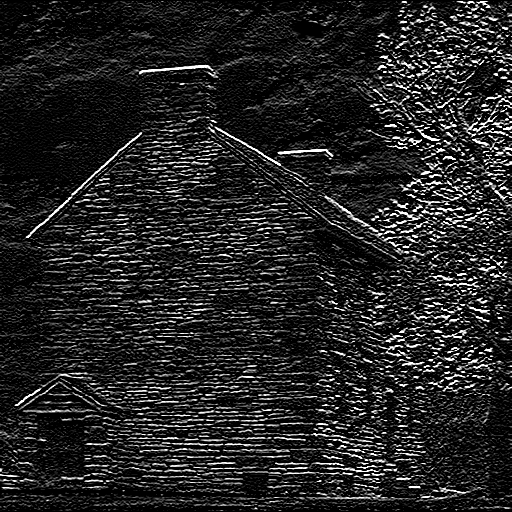
\includegraphics[width=0.9\textwidth]{imagens/house.png}
        \caption{Original: \texttt{house.png}.}
        \label{fig:blur:orig}
    \end{subfigure}\\[8pt]
    \begin{subfigure}{0.48\textwidth}
        \centering
        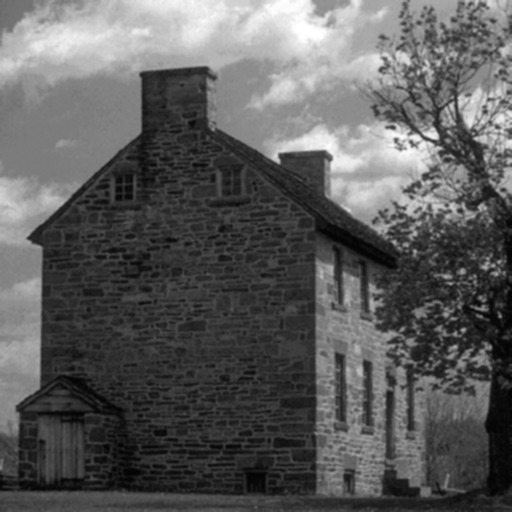
\includegraphics[width=0.9\textwidth]{resultados/house_h2.png}
        \caption{Convolução com $h_2$ (\ref{fig:h2}).}
        \label{fig:blur:gauss}
    \end{subfigure}%
    \begin{subfigure}{0.48\textwidth}
        \centering
        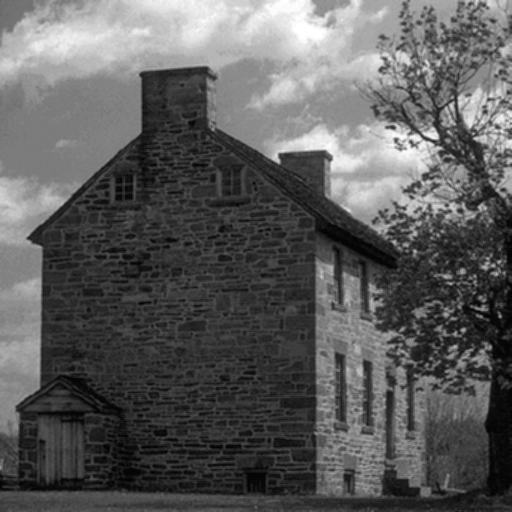
\includegraphics[width=0.9\textwidth]{resultados/house_h6.png}
        \caption{Convolução com $h_6$ (\ref{fig:h6}).}
        \label{fig:blur:box}
    \end{subfigure}

    \caption{Aplicação do \textit{blur}.}
    \label{fig:blur}
\end{figure}

O segundo filtro é chamada de \textit{box blur}, que faz uma média simples da vizinhaça 8 do pixel. Isso pode ser visto no \textit{kernel} do filtro (\cref{fig:h6}). Apesar de ser diferente do gaussiano, o resultado ficou bem parecido, como pode ser visto na \cref{fig:blur}. O motivo disso é que os pesos mais externos do filtro gaussiano $5 \times 5$ são bem baixos, fazendo com a região $3 \times 3$ seja mais presente, sendo essa a mesma região do filtro \textit{box}.

No programa, esses filtros podem ser aplicados com \mintinline[breaklines]{bash}{python3 main.py imagens/house.png h2} ~ou~ \mintinline[breaklines]{bash}{python3 main.py imagens/house.png h6}.
